\section[相似变换]{相似变换\\Similarity Transformations}	
\par\noindent
在前面的章节中,我们通过增益矩阵$G$解决$A^\mathsf{T}A$秩亏的问题。同时,我们对最小二乘做了约束。这些约束也通过$G$描述!然而,约束可能更是一种通用式形式。在这一章节中,我们将会
介绍将自由网转换为至少具有$d$个假设坐标的网,我们也将会推导出相关的公式。相关的协方差矩阵$\sum_{transformed}$将会作出相关改变,$d$列与行通常将会被赋值为0。我们通过解决一个简单
的例题开始。
\begin{figure}
	\centering
	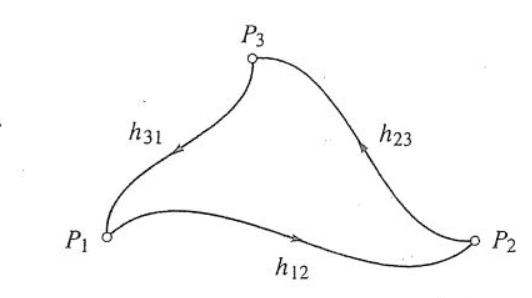
\includegraphics[width=0.4\linewidth]{TeX_files/Part02/chapter07/image/7-4}
	\caption{图7.4  简单自由水准网}
	\label{fig:7-4}
\end{figure}

\par\noindent
\textbf{例7.6} 如图7.4,一个简单的自由水准网$A$有三个节点$P_1$ ,$P_2$,和$P_3$并且观测到了不同方向的高差$h_{12}$, $h_{23}$,和$h_{31}$。根据循环律我们得到
\begin{equation}
	h_{12} + h_{23} + h_{31} = 0 \text{。}
\end{equation}
利用这些高差我们不能计算出节点的高程。因此,我们选择$P_1$作为参考点。我们令$P_1$ =常量 = $h_1$。$h_2$ 和 $h_3$的最佳估计值现在是唯一的
\begin{equation}
	h_{i} = h_{1i} + h_{1} = h_{i}^{1} + h_1,\qquad i = 1,2,3
\end{equation}
公式中上标指的是已选择的参考点。然而这里有一个轻微的缺陷,即选择了任意点$P_1$作为参考。实际上,我们可以选择网中的任意一个点作为参考点。我们甚至可以选择质心$P_b$并且将它的高程
赋值为\begin{equation*}
	h_{b} = \frac{1}{n}\sum_{i = 1}^{n}h_i \text{。}
\end{equation*}
这导致
\begin{equation*}
	h_{i} = \frac{1}{3}(h_{1i} + h_{2i} + h_{3i}) + h_b = h_{i}^{b} + h_b \text{。}
\end{equation*}
所有组的高差像是$h_{i}^{1}$和$h_{i}^{b}$都可以视为有效高差。因此它更像是一个选择哪组高差的问题。然而高差$h_{i}^{1}$ 或者$h_{i}^{b}$的统计特性很大程度上依赖于参考点的选择。例
如,从$E{h_{3}^{1}} = E{h_{3}^{1} + h_{2}^{3}}$ 和$E{h_{3}^{b}} = E{\frac{2}{3}h_{1}^{2} + h_{2}^{3} + \frac{1}{3}h_{1}^{3}}$可得出$E{h_{3}^{1}} \neq E{h_{3}^{b}}$。它们的协方
差也是不同的。
\par
当比较两组高程时,他们具有相同参考水平是重要的。因此为了能够比较两组高程,我们应该学会如何将高程从一个系统转换到另外一个系统。我们明确地写出式(7.28)
\begin{equation}
	\begin{bmatrix}
		h_{1}\\
		h_{2}\\
		h_{3}
	\end{bmatrix}
	= \begin{bmatrix}
		h_{1}^{1}\\
		h_{2}^{1}\\
		h_{3}^{1}
	\end{bmatrix}
	+ \begin{bmatrix}
		1 & 0 & 0\\
		1 & 0 & 0\\
		1 & 0 & 0
	\end{bmatrix}
	\begin{bmatrix}
		h_{1}\\
		h_{1}\\
		h_{1}
	\end{bmatrix}
\end{equation}
或\begin{equation}
	\begin{bmatrix}
		h_{1}^{1}\\
		h_{2}^{1}\\
		h_{3}^{1}
	\end{bmatrix}
	=\begin{bmatrix}
		\quad0 & \quad0 & \quad0\\
		-1 & \quad1 & \quad0\\
		-1 & \quad0 & \quad1
	\end{bmatrix}
	\begin{bmatrix}
		h_{1}\\
		h_{2}\\
		h_{3}
	\end{bmatrix}\text{。}
\end{equation}
式(7.30)展示给我们如何转换一个高程系统,例如将$h_{i}^{1}$转换到由 $P_1$作为参考点定义的高程系统。以同样的方式我们得到
\begin{equation*}
	\begin{bmatrix}
		h_{1}^{b}\\
		h_{2}^{b}\\
		h_{3}^{b}
	\end{bmatrix}
	=\frac{1}{3}
	\begin{bmatrix}
		\quad2 & -1 & -1\\
		-1 & 2 & -1\\
		-1 & -1 & \quad2
	\end{bmatrix}
	\begin{bmatrix}
		h_{1}^{1}\\
		h_{2}^{1}\\
		h_{3}^{1}
	\end{bmatrix}
\end{equation*}
通常
\begin{equation}
	\begin{bmatrix}
		h_{1}^{b}\\
		h_{2}^{b}\\
		\vdots\\
		h_{n}^{b}
	\end{bmatrix}
	=\frac{1}{n}
	\begin{bmatrix}
		n - 1 & -1 & \ldots&-1\\
		-1 &  n - 1& \ldots&-1\\
		\vdots&\vdots&\ddots&\vdots\\
		-1 & -1 &\ldots&   n - 1
	\end{bmatrix}
	\begin{bmatrix}
		h_{1}^{1}\\
		h_{2}^{1}\\
		\vdots\\
		h_{n}^{1}
	\end{bmatrix}\text{。}
\end{equation}
当$n = 5$时,这个方阵就是例7.3中的方阵。
\par
这个二维的转换模型需要两个平移参数$t_x$,$ t_y$,一个旋转参数$r_\varphi$和一个尺度参数$s_k$。从$(x , y)$到$(\xi, \eta)$的\emph{相似变换}(在大地测量中“从”和“到”系统)由下式给出
\begin{equation}
	\begin{bmatrix}
		\xi_{i}\\
		\eta_{i}
	\end{bmatrix}
	= k
	\begin{bmatrix}
		\ \cos\varphi & \sin \varphi\\
		-\sin \varphi & \cos \varphi
	\end{bmatrix}
	\begin{bmatrix}
		x_i\\
		y_i
	\end{bmatrix}
	+   \begin{bmatrix}
		t_x\\
		t_y
	\end{bmatrix}\text{。}
\end{equation}
式(7.32)并不是关于$\varphi$ 的线性函数,但是我们可以巧妙地使它线性化。引进新的松弛变量$a = k \cos \varphi$和$b = \sin \varphi$,得到
\begin{equation}
	\begin{bmatrix}
		\xi_{i}\\
		\eta_{i}
	\end{bmatrix}
	=
	\begin{bmatrix}
		\ a & b\\
		-b & a
	\end{bmatrix}
	\begin{bmatrix}
		x_i\\
		y_i
	\end{bmatrix}
	+   \begin{bmatrix}
		t_x\\
		t_y
	\end{bmatrix}\text{。}
\end{equation}
由$p$个公共点组成的$2p$个观测方程是
\begin{equation}
	\begin{bmatrix}
		x_1 & y_1 & 1 & 0\\
		x_2 & y_2 & 1 & 0\\
		&\vdots\\
		x_p & y_p & 1 & 0\\
		y_1 &-x_1 & 0 & 1\\
		y_2 &-x_2 & 0 & 1\\
		&\vdots\\
		y_p &-x_p & 0 & 1
	\end{bmatrix}
	\begin{bmatrix}
		a\\
		b\\
		t_x\\
		t_y
	\end{bmatrix}
	=
	\begin{bmatrix}
		\xi_1\\
		\xi_2\\
		\vdots\\
		\xi_p\\
		\eta_1\\
		\eta_2\\
		\vdots\\
		\eta_p
	\end{bmatrix}
	-
	\begin{bmatrix}
		e\xi_1\\
		e\xi_2\\
		\vdots\\
		e\xi_p\\
		e \eta_1\\
		e\eta_2\\
		\vdots\\
		e\eta_p
	\end{bmatrix}\text{。}
\end{equation}
或者可以象征地表示为
\begin{equation*}
	Af = b - e \text{。}
\end{equation*}
线性最小二乘问题很简单。
\par
然而我们不能不了解证明经典求解的过程。我们设置等价权并且法方程$A^\mathsf{T}Af = A^\mathsf{T}b$可以被写为
\begin{equation}
	\begin{bmatrix}
		\sum(x_{i}^{2} + y_{i}^{2}) & 0 & \sum x_i & \sum y_i\\
		0 & \sum(x_{i}^{2} + y_{i}^{2}) & \sum y_i & -\sum x_i\\
		\sum x_i & \sum y_i & p & 0\\
		\sum y_i &-\sum x_i & 0 & p
	\end{bmatrix}
	\begin{bmatrix}
		a\\
		b\\
		t_x\\
		t_y
	\end{bmatrix}
	=
	\begin{bmatrix}
		\sum(\xi_ix_i + \eta_iy_i)\\
		\sum(\xi_iy_i - \eta_ix_i\\
		\sum\xi_i\\
		\eta_i
	\end{bmatrix}\text{。}
\end{equation}
包括从点1到点$p$的所有点。由于数值原因,我们将两个系统的坐标归纳到它们各自的重心$(x_s, y_s)$ 和$(\xi_s, \eta_s)$。这导致 $\sum_{x_i} = \sum_{y_i} = \sum_{\xi_i} = 
\sum_{\eta_i} \equiv 0$ 和 $A^\mathsf{T}A$成为对角阵。我们引入与重心相关的带有星级标志的坐标$x_{i}^{*} = x_i - x_s, y_{i}^{*} = y_i - y_s$,其中$x_s = \sum x_i/p, y_s = \sum 
y_i/p$:
\par
现在求逆就转换为求解单个方程:
\begin{equation*}
	\begin{bmatrix}
		\star & 0 & 0 & 0\\
		0 & \star & 0 & 0\\
		0 & 0 & p & 0\\
		0 & 0 &0 & p
	\end{bmatrix}
	\begin{bmatrix}
		a\\
		b\\
		t_x\\
		t_y
	\end{bmatrix}
	=
	\begin{bmatrix}
		\star\\
		\star\\
		0\\
		0
	\end{bmatrix}\text{。}
\end{equation*}
非零的项用$\star$标记。确定的解可被写为
\begin{equation}
	\hat{a} = \frac{\sum(\xi_{i}^{\ast} x_{i}^{\ast} + \eta_{i}^{\ast} y_{i}^{\ast})}
	{\sum{(x_{i}^{\ast}}^{2}  + {y_{i}^{\ast}}^{2})}
	\qquad \text{和} \qquad
	\hat{b} = \frac{\sum(\xi_{i}^{\ast} y_{i}^{\ast} - \eta_{i}^{\ast} x_{i}^{\ast})}
	{\sum{(x_{i}^{\ast}}^{2}  + {y_{i}^{\ast}}^{2})}\text{。}
\end{equation}
下面,我们可以确定
\begin{equation}
	\hat{k} = \sqrt{{\hat{a}}^2 + {\hat{b}}^2}
	\qquad \text{and} \qquad
	\hat{\varphi} = \arctan{\hat{b} / \hat{a}}\text{。}
\end{equation}
最终,我们可以从(7.34)得到$\hat{t}_x$和$\hat{t}_y$:
\begin{equation}
	\hat{t}_x = \frac{\sum \xi_i - \hat{a}\sum x_i - \hat{b}\sum y_i}{p}
	= \xi_s - \hat{a}x_s - \hat{b}y_s,
\end{equation}
\begin{equation}
	\hat{t}_y = \frac{\sum \eta_i - \hat{a}\sum y_i + \hat{b}\sum x_i}{p}
	= \eta_s - \hat{a}y_s + \hat{b}x_s\text{。}
\end{equation}
$\hat{f}$协方差矩阵包含 $A = p\sum(x_{i}^{2} + y_{i}^{2})
- (\sum x_{i})^{2}- (\sum y_{i})^{2}$ :
\begin{equation*}
	\sum\nolimits_{\hat{f}} = \frac{1}{A}
	\begin{bmatrix}
		\ p       & \ 0        & -\sum x_i                      &-\sum y_i\\
		\ 0       & \ p        & \ -\sum y_i                    &\ \sum x_i\\
		-\sum x_i & -\sum y_i  & \ \sum(x_{i}^{2} + y_{i}^{2})  &\ 0\\
		-\sum y_i & \ \sum x_i & \ 0                            &\ \sum(x_{i}^{2} + y_{i}^{2})
	\end{bmatrix}\text{。}
\end{equation*}
单位权的方差也是转换坐标的方差。根据式(4.79)
\begin{equation*}
	\hat{\sigma}_{0}^{2} = \frac{\sum(e_{\xi_i}^{2} + e_{\eta_i}^{2})}{2p - 4}\text{。}
\end{equation*}
由于平移我们得到
\begin{equation}
	\hat{\sigma}_{\hat{t}_x} = \hat{\sigma}_{\hat{t}_y}
	= \hat{\sigma}_0\sqrt{\frac{\sum(x_{i}^{2} + y_{i}^{2})}{p\sum(x_{i}^{2} + y_{i}^{2})
			- (\sum x_{i})^{2} - (\sum y_{i})^{2}}}
	= \hat{\sigma}_0\sqrt{\frac{1}{p} + \frac{x_{s}^{2} + y_{s}^{2}}{{\sum({x_{i}^\ast}}^{2} + {y_{i}^{\ast}}^{2})}}\text{。}
\end{equation}
观察到$\hat{t}_x$和$\hat{t}_y$的标准差不仅仅不出所料的取决于$p$,而且也取决于原点的位置。
\par
因此我们已经描述了关于相似变换的最重要、最基本的情况。它包含$p$个点,这$p$个点的坐标在两个系统中都被给出,即一个原始的$x$,$y$系统和一个不同的$\xi$,$\eta$系统。通过一个最小二
乘过程求解转换参数$\hat{k}$, $\hat{\varphi}$, $\hat{t}_x$ 和 $\hat{t}_y$。此外,通过\emph{转换方程},该方法可将其它任何点$(x_j,y_j)$转换为相应的$(\xi_i,\eta_j)$
\begin{equation}
	\xi_j
	= \hat{a}x_j + \hat{b}y_{j} + \hat{t}_x,\qquad
	\eta_j = -\hat{b}x_j + \hat{a}y_{j} + \hat{t}_y\text{。}
\end{equation}
\textbf{例7.7}  我们仅通过一个数值实例演示该过程。假设我们知道7个公共点的准确坐标$(N, E) = (\xi, \eta)$和$(X, Y)$。我们想要确定转换参数并且转换一个被给出$x, y$坐标的点。这个实
际上是一个二维插值的过程。
\par
\begin{table}[htbp]
	% \caption{\label{tab:test}}
	\begin{tabular}{ccccc}
		\toprule
		\multirow{2}{*}{Point} & $x_i$ & $y_i$ & $\xi_{i}$ & $\eta_i$ \\
		{} &[m] & [m] & [m] & [m]\\
		\midrule
		62-04-005 &277 722.022  &-230 855.152 & 6 310 000.527 &562 940.820\\
		62-04-801 &275 956.869  &-231 105.839 & 6 308 231.260 &562 725.625\\
		62-04-810 &277 563.374  &-235 447.400 & 6 309 749.964 &558 354.121\\
		62-04-811 &278 608.525  &-233 945.915 & 6 310 824.656 &559 833.890\\
		62-04-815 &276 163.682  &-236 471.626 & 6 308 330.475 &557 358.463\\
		63-01-002 &273 578,801  &-230 941.425 & 6 305 857.705 &562 937.589\\
		63-04-003 &274 533.958  &-235 063.723 & 6 306 729.799 &558 798.283\\
		$s$       &276 303.890  &-233 404.440 & 6 308 532.055 &560 421.256\\
		\bottomrule
	\end{tabular}
\end{table}
\begin{table}[htbp]
	% \caption{\label{tab:test}}
	\begin{tabular}{ccccc}
		\toprule
		\multirow{2}{*}{Point} & $x_{i}^{\ast}$ & $y_{i}^{\ast}$ & $\xi_{i}^{\ast}$ & $\eta_{i}^{\ast}$ \\
		{} &[m] & [m] & [m] & [m]\\
		\midrule
		62-04-005 &\ 1 418.132  &\ 2 549.288  &\ 1 468.472 &\ 2 519.564\\
		62-04-801 &-347.021     &\ 2 298.601  & -300.795   &\ 2 304.369\\
		62-04-810 &\ 1 259.484  & -2 042.960  &1\ 217.909  &-2 067.135\\
		62-04-811 &\ 2 304.635  &-541.475     &\ 292.601   &-5 87.366\\
		62-04-815 &-140.208     &-3 067.186   &-201.580    &-3 062.793\\
		63-01-002 &-2 725.089   &\ 2 463.015  &-2674.350   &\ 2 516.333\\
		63-04-003 &-1 769.932   &-1 659.283   &-1802.256   &-1 622.973\\
		Sum       &\ .001       &\ .000       &\ .001      &\ .001\\
		\bottomrule
	\end{tabular}
\end{table}
\par
首先,我们列出假定坐标。点$s$是重心(它的坐标在最后一行)。第二张表给出了转化到重心的相同数据。后者用$\ast$标记。
产品的必要总数是
\begin{equation*}
	\sum{{x_{i}^\ast}}^{2} = 19 607 592.00 \qquad \sum{{y_{i}^\ast}}^{2} = 34476 609.52
\end{equation*}
\begin{equation*}
	\sum x_{i}^{\ast}\eta_{i}^{\ast} = -4739 029.25 \qquad \sum y_{i}^{\ast}\xi_{i}^{\ast} =  -3 655 603.21
\end{equation*}
\begin{equation*}
	\sum x_{i}^{\ast}\xi_{i}^{\ast} = 19 510390.19 \qquad \sum y_{i}^{\ast}\eta_{i}^{\ast} = 34 545 930.52
\end{equation*}
\begin{equation*}
	\hat{a} = 0.99948449 \qquad \hat{b} = 0.020032 21
\end{equation*}
\begin{equation*}
	\hat{k} = 0.999 685 22 \qquad \hat{\varphi} = 1.275 777 \text{gon}
\end{equation*}
\begin{equation*}
	\hat{t}_x = \xi_s - \hat{a}x_s - \hat{b}y_s = 6 037 046.208
\end{equation*}
\begin{equation*}
	\hat{t}_y = \eta_s + \hat{b}x_s - \hat{a}y_s = 6 037 046.208
\end{equation*}\text{。}
\par
$(x_j, y_j)$到$(\xi_j, \eta_j)$的转换方程式(7.40)包括一次旋转和一次平移:
\par $\xi_j = 0.999 484 49 x_j + 0.020 032 21 y_j + 6 037 046.208$
\par $\eta_j = -0.020 032 21 x_j + 0.999 484 49 y_j + 799 240.351.$
\par\noindent
具有坐标$(x, y) = (276 109.847, — 233 507.185)$的点被转换为$(\xi, \eta) =(6308 336.054, 560322.451)$。官方值是(6 308336.054, 560322.449),显然,精度是符合要求的。这其中一部分
的原因是转换的点接近重心。通过$M$样文件,我们得到$\hat{\sigma}_0 = 3$mm。
\par
\emph{这个过程被称为赫尔默特转换}。思考周到的读者可能会问为什么在变换过程中我们让公共点的坐标$(x_i, y_i)$不会改变。公式化有利于上面的一个点集,以便于它们没有假定误差,假定坐标
$(x_i, y_i)$比$(\xi_i, \eta_i)$会更好吗?实际上,当这些点$(\xi_i, \eta_i)$在此过程中单独调整的时候,这些点$(x_i, y_i)$作为“固定”点组被转换。因此,为什么不允许两个点集在转换中
调整?事实上坐标$(x_i, y_i)$比新计算的坐标$(\xi_i, \eta_i)$更不好。因此,用两种其它类型的观测方程增强式(7.32),相关公式为
\begin{equation}
	\begin{bmatrix}
		\xi_i\\
		\eta_i\\
		X_{i}^{'}\\
		Y_{i}^{'}
	\end{bmatrix}
	\begin{bmatrix}
		a  & b\\
		-b & a\\
		1 & 0\\
		0 & 1
	\end{bmatrix}
	\begin{bmatrix}
		x_i\\
		y_i
	\end{bmatrix}
	+
	\begin{bmatrix}
		t_x\\
		t_y\\
		0\\
		0
	\end{bmatrix}\text{。}
\end{equation}
其中$(\xi_i, \eta_i)$和$(X_{i}^{'},Y_{i}^{'})$表示两个系统中公共点的假定坐标。但是也已经发生了一个值得注意的变化:$p$组$(x_i, y_i)$已经作为附加的未知数被引进,与之前的4个未知数
$a$ $b$,$t_x$,$t_y$一起被估算。
\par
我们只是引用了在Teunissen (1985b), 141-146中给出的结果。尺度通过更复杂的表达式$\hat{k} = \lambda + \sqrt{1 + \lambda^2}$表示。其中
\begin{equation*}
	\lambda =  \frac{\sum({\xi_{i}^{\ast}}^2 + {\eta_{i}^{\ast}}^2) - \sum({X_{i}^{'}}^{\ast2} + {Y_{i}^{'}}^{\ast2})}
	{\sqrt[2]{(\sum\xi_{i}^{\ast}{X_{i}^{'}}^{\ast} + \eta_{i}^{\ast}{Y_{i}^{'}}^{\ast})^{2} + (\sum\xi_{i}^{\ast}{Y_{i}^{'}}^{\ast} - \eta_{i}^{\ast}{X_{i}^{'}}^{\ast})^{2}}}
\end{equation*}
\begin{equation*}
	X_s =  \frac{1}{n}\sum X_{i}^{'},\quad  Y_s = \frac{1}{n}\sum Y_{i}^{'},\quad {X_{i}^{'}}^{\ast} = X_s - X_{i}^{i},\quad  {Y_{i}^{'}}^{\ast} = Y_s - Y_{i}^{i}
\end{equation*}
\begin{equation}
	\hat{\varphi} = \arctan{\frac{\sum \xi_{i}^{\ast}{Y_{i}^{'}}^{\ast} - \eta_{i}^{\ast}{X_{i}^{'}}^{\ast}}{\sum \xi_{i}^{\ast}{X_{i}^{'}}^{\ast} - 
			\eta_{i}^{\ast}{Y_{i}^{'}}^{\ast}}}
\end{equation}
\begin{equation*}
	\hat{t}_x = x_s - X_s\hat{k}\cos{\hat{\varphi}} - Y_s\hat{k}\sin{\hat{\varphi}}
\end{equation*}
\begin{equation*}
	\hat{t}_y = y_s + X_s\hat{k}\sin{\hat{\varphi}} - Y_s\hat{k}\cos{\hat{\varphi}}
\end{equation*}
\begin{equation*}
	\hat{x}_i = X_s + \frac{1}{1 + \hat{k}^2}({X_{i}^{'}}^\ast + \xi_{i}^{\ast}\hat{k}\cos\hat{\varphi} - \eta_{i}^{\ast}\hat{k}\sin\hat{\varphi})
\end{equation*}
\begin{equation*}
	\hat{y}_i =
	Y_s + \frac{1}{1 + \hat{k}^2}({Y_{i}^{'}}^\ast + \xi_{i}^{\ast}\hat{k}\sin\hat{\varphi} - \eta_{i}^{\ast}\hat{k}\cos\hat{\varphi})
\end{equation*}

比较$\hat{k} = \lambda + \sqrt{1 + \lambda^2}$和表达式 $\hat{k} = \sqrt{\hat{a}^2 + \hat{b}^2}$(其中$\hat{a}$和$\hat{b}$由式(7.35)给出)比较得出:后面的表达式与由式(7.42) 
给出的值相比系统地低估了该尺度。
\par
当两组公共点的坐标被调整,这个模型就不再是线性的并且我们得到了$\hat{k}$的有偏估计。旋转参数$\hat{\varphi}$ 和平移参数$\hat{t}_x$、$\hat{t}_y$仍然是无偏估计。$\hat{k}$的\
emph{偏差}可以通过下式体现
\begin{equation}
	b_{\hat{k}}
	= 3\frac{1 + \hat{k}^2}{(n - 1)n\hat{k}}\frac{\hat{\sigma_{0}^{2}}}{d^2}
\end{equation}
其中,公共点被放置于边长为$d$的方格子中。表达式(7.43)表明对于大部分的实际问题偏差是可以忽略。如果 $\hat{\sigma}_0/d = 10^{-5}$,$\hat{k} = 1$,和$n = 4$我们得到$b_{\hat{k}} = 
0.5 \times 10^{-10}$。
\par
例子是有趣的,因为即使是一个简单的非线性最小二乘问题都可以引进未知数有偏估计。